\documentclass[conference]{IEEEtran}
\usepackage[utf8]{inputenc} % Add Unicode support
\usepackage{graphicx}
\usepackage[greek,english]{babel} % Support for Greek language
\bibliographystyle{IEEEtran}
\begin{document}
\selectlanguage{greek} % Select Greek for this part of the document

\title{\textlatin{Xception \& GRU} για δημιουργια περιγραφής σε εικόνες}
\author{
    \IEEEauthorblockN{Παπαγρηγορίου Βασίλειος Σάββας}
    \IEEEauthorblockA{
        \textlatin{vasilispapg@outlook.com} \\
        \textit{Π.Μ.Σ. Τεχνητή Νοημοσύνη} \\
        \textit{Α.Π.Θ.}
    }
}

\maketitle

\section{Εισαγωγή}
Αυτό που προσπάθησα αρχικά ηταν η κατανοηση των συνελεκτικων δικτυων ωστε να βρω τρόπο να παραγω κάποια στοιχεία τα οποια θα έχουν σημασία για τα αναδρομικά δίκτυα. Ξεκίνησα με απλά συνελεκτικα δίκτυα ενός ή δύο \textlatin{layer} και στην συνέχεια προσπαθησα να χρησιμοποιησω καποιες αρχιτεκτονικές όπως \textlatin{ResNet-50}, \textlatin{Xception}. Για τα αναδορμικά δίκτυα ξεκίνησα με \textlatin{RNN} και στην συνεχεια προσπαθησα να εφαμορσω μια τεχνική που διαβασα σε ενα προσφατο \textlatin{paper} για το \textlatin{patch and pack} με \textlatin{Visual Transformers (NaViT)} τα οποια παιρνουν εικονες οποιαδηποτε μεγεθους. Αλλά, μας είπατε οτι αυτα απαιτουν πολλους πορους για να εκπαιδευτουν, άλλαξα τακτική και πήγα σε μια πιο απλή λύση με την χρήση των \textlatin{LSTM} και στην συνέχεια με την χρήση των \textlatin{Positional Encodings}. Στο τέλος, κατέληξα με το σύστημα ενός προ-εκπαιδευμένουν \textlatin{Xception} για την εξαγωγή των χαρακτηριστικών και με την χρήση των \textlatin{GRU} δικτύου για την δημιουργία τω περιγραφών. Για δεδομένα χρησιμοποίησα το \textlatin{dataset} του \textlatin{Flickr8k} απο το \textlatin{kaggle}.

\section{Προεπεξεργασία Δεδομένων}

Η προεπεξεργασία δεδομένων αποτελεί κρίσιμο στάδιο στην ανάπτυξη και εκπαίδευση των μοντέλων μηχανικής μάθησης. Στο πλαίσιο της εργασίας αυτής, η προεπεξεργασία των δεδομένων πραγματοποιήθηκε ως εξής:

\subsection{Σύνολο Δεδομένων}
Χρησιμοποιήθηκε το σύνολο δεδομένων \textlatin{Flickr8k}, το οποίο περιλαμβάνει 8.000 εικόνες με περιγραφές (λεζάντες) στα Αγγλικά. Κάθε εικόνα συνοδεύεται από πέντε διαφορετικές περιγραφές που περιγράφουν την εικόνα. Αυτό το σύνολο δεδομένων είναι ευρέως χρησιμοποιούμενο για την εκπαίδευση και αξιολόγηση μοντέλων περιγραφής εικόνας.

\subsection{\textlatin{Tokenization}}
Για την επεξεργασία των περιγραφών, χρησιμοποιήθηκε η βιβλιοθήκη \textlatin{\texttt{spacy}} για την ανάλυση και διαχωρισμό των προτάσεων σε λέξεις \textlatin{(tokens)}. Η διαδικασία της tokenization είναι σημαντική για τη μετατροπή των κειμένων σε μορφή που μπορεί να επεξεργαστεί το μοντέλο.

\subsection{Δημιουργία Λεξιλογίου}
Η επόμενη φάση περιλάμβανε τη δημιουργία ενός λεξιλογίου από τις περιγραφές του συνόλου δεδομένων. Το λεξιλόγιο περιλαμβάνει όλες τις μοναδικές λέξεις που εμφανίζονται στις περιγραφές, με συχνότητα εμφάνισης πάνω από ένα προκαθορισμένο κατώφλι. Λέξεις με πολύ χαμηλή συχνότητα εμφάνισης εξαιρέθηκαν για να μειωθεί η πολυπλοκότητα του μοντέλου.

\subsection{Μετατροπή σε Αριθμητικές Τιμές \textlatin{(Numericalization)}}
Μετά την δημιουργία του λεξιλογίου, οι λέξεις στις περιγραφές μετατράπηκαν σε αριθμητικές τιμές, χρησιμοποιώντας ένα σύστημα αντιστοίχισης λέξεων σε μοναδικούς αριθμούς. Αυτή η διαδικασία είναι γνωστή ως \textlatin{numericalization} και επιτρέπει στο μοντέλο να επεξεργαστεί τις λέξεις ως αριθμητικά δεδομένα.

\subsection{Μετασχηματισμοί Εικόνων}
Για την επεξεργασία των εικόνων, εφαρμόστηκαν διάφοροι μετασχηματισμοί ώστε να διασφαλιστεί η ομοιογένεια και η κανονικοποίηση των δεδομένων εισόδου. Αυτοί οι μετασχηματισμοί περιλαμβάνουν την αλλαγή μεγέθους των εικόνων σε συγκεκριμένες διαστάσεις και την κανονικοποίηση των τιμών των pixel με βάση τη μέση και τυπική απόκλιση των τιμών των pixel στο σύνολο δεδομένων \textlatin{ImageNet}.

\subsection{Προεπεξεργασία των Περιγραφών}
Οι περιγραφές προεπεξεργάστηκαν ώστε να αφαιρεθούν μη αλφαβητικοί χαρακτήρες και λέξεις με ένα μόνο χαρακτήρα. Επιπλέον, προστέθηκαν ειδικά tokens έναρξης και λήξης (<\textlatin{start}> και <\textlatin{end}>) σε κάθε περιγραφή, καθώς και padding για να εξασφαλιστεί ότι όλες οι περιγραφές έχουν το ίδιο μήκος.


\section{Αρχιτεκτονική Μοντέλου}

Η αρχιτεκτονική του μοντέλου αποτελείται από έναν \textlatin{Encoder} και έναν \textlatin{Decoder} που συνεργάζονται για να παράγουν περιγραφές εικόνας.

\subsection{\textlatin{Encoder} (Κωδικοποιητής)}

Ο \textlatin{Encoder} είναι υπεύθυνος για την επεξεργασία των χαρακτηριστικών των εικόνων. Η αρχιτεκτονική του \textlatin{Encoder} περιλαμβάνει τα εξής στάδια:

\begin{itemize}
    \item \textbf{Προβολή Χαρακτηριστικών}: Τα χαρακτηριστικά της εικόνας που εξάγονται από το οπτικό μοντέλο (όπως το \textlatin{Xception}) περνούν από ένα επίπεδο προβολής που τα μετατρέπει σε έναν νέο χώρο ενσωμάτωσης (\textlatin{embedding space}).
    \item \textbf{Διαμόρφωση Διάστασης}: Οι διαστάσεις της εισόδου προσαρμόζονται ώστε να είναι συμβατές με τις απαιτήσεις του \textlatin{GRU}.
\end{itemize}

\subsection{\textlatin{Decoder} (Αποκωδικοποιητής)}

Ο \textlatin{Decoder} είναι υπεύθυνος για την παραγωγή της τελικής περιγραφής της εικόνας. Η αρχιτεκτονική του \textlatin{Decoder} περιλαμβάνει τα εξής στάδια:

\begin{itemize}
    \item \textbf{Ενσωμάτωση Λέξεων}: Οι λέξεις της περιγραφής μετατρέπονται σε διανύσματα ενσωμάτωσης (\textlatin{embedding vectors}) μέσω ενός επιπέδου ενσωμάτωσης.
    \item \textbf{\textlatin{GRU}}: Χρησιμοποιείται μια μονάδα \textlatin{GRU} για την επεξεργασία των ενσωματωμένων διανυσμάτων και την παραγωγή της τελικής περιγραφής.
    \item \textbf{Τελικό Γραμμικό Επίπεδο}: Ένα τελικό γραμμικό επίπεδο χρησιμοποιείται για να προβλέψει την πιθανότητα κάθε λέξης στο λεξιλόγιο.
\end{itemize}

\subsection{\textlatin{Image Captioning Model}}

Το τελικό μοντέλο περιγραφής εικόνας (\textlatin{Image Captioning Model}) συνδυάζει τον \textlatin{Encoder} και τον \textlatin{Decoder} για να παράγει περιγραφές εικόνων. Η αρχιτεκτονική περιλαμβάνει τα εξής:

\begin{itemize}
    \item \textbf{Οπτικό Μοντέλο (\textlatin{Visual Model})}: Χρησιμοποιείται το \textlatin{Xception} για την εξαγωγή χαρακτηριστικών από τις εικόνες.
    \item \textbf{\textlatin{Encoder}}: Ο \textlatin{Encoder} λαμβάνει τα χαρακτηριστικά της εικόνας και τα προβάλλει σε έναν χώρο ενσωμάτωσης.
    \item \textbf{\textlatin{Decoder}}: Ο \textlatin{Decoder} λαμβάνει τα ενσωματωμένα διανύσματα και τις εισόδους των περιγραφών για να παράγει την τελική περιγραφή της εικόνας.
\end{itemize}

\section{Εκπαίδευση}

Η εκπαίδευση του μοντέλου αποτελεί κρίσιμο στάδιο για την επίτευξη υψηλής απόδοσης και ακρίβειας. Η διαδικασία εκπαίδευσης περιλαμβάνει διάφορα βήματα και τεχνικές που εφαρμόστηκαν για την βελτιστοποίηση του μοντέλου.

\subsection{Βρόχος Εκπαίδευσης}

Ο βρόχος εκπαίδευσης (\textlatin{training loop}) που χρησιμοποιήθηκε για την εκπαίδευση του μοντέλου περιλαμβάνει τα εξής βήματα:

\begin{itemize}
    \item \textbf{Προετοιμασία Δεδομένων}: Τα δεδομένα χωρίζονται σε σύνολα εκπαίδευσης και επικύρωσης. Χρησιμοποιήθηκε η συνάρτηση \textlatin{SplitDataset} για να δημιουργήσει τα σύνολα δεδομένων και τους αντίστοιχους φορτωτές (\textlatin{data loaders}).
    \item \textbf{Ορισμός Μοντέλου και Βελτιστοποιητή}: Το μοντέλο \textlatin{ImageCaptioningModel} ορίζεται και μεταφέρεται στη συσκευή (\textlatin{device}) εκπαίδευσης. Χρησιμοποιήθηκε κυρίως ο βελτιστοποιητής \textlatin{Adam} με διάφορες υπερπαραμέτρους, αλλά επίσης δοκιμάστηκαν και οι \textlatin{Adagrad} και \textlatin{SGD}.
    \item \textbf{Ορισμός Κριτηρίου}: Ως κριτήριο απώλειας (\textlatin{criterion}) χρησιμοποιήθηκε η \textlatin{Cross-Entropy Loss} με μάσκα για την αντιμετώπιση των τιμών \textlatin{padding}.
    \item \textbf{Αξιολόγηση}: Μετά από κάθε εποχή, το μοντέλο αξιολογείται στο σύνολο δεδομένων επικύρωσης για να παρακολουθηθεί η απόδοσή του και να εντοπιστούν πιθανά προβλήματα υπερεκπαίδευσης.
    \item \textbf{Αποθήκευση Προτύπου}: Ανά τακτά διαστήματα, το πρότυπο αποθηκεύεται για να διασφαλιστεί ότι οι παράμετροι του μοντέλου διατηρούνται.
\end{itemize}

\subsection{Κώδικας Εκπαίδευσης}

Ο κώδικας εκπαίδευσης περιλαμβάνει τις εξής λειτουργίες:

\begin{itemize}
    \item \textbf{\textlatin{SplitDataset}}: Χωρίζει το σύνολο δεδομένων σε υποσύνολα εκπαίδευσης και επικύρωσης και δημιουργεί φορτωτές δεδομένων.
    \item \textbf{\textlatin{get\_arguments}}: Λαμβάνει τα επιχειρήματα γραμμής εντολών για να καθορίσει τις λειτουργίες που θα εκτελεστούν (εκπαίδευση, πρόβλεψη, αξιολόγηση, κ.λπ.).
    \item \textbf{\textlatin{train\_model}}: Εκπαιδεύει το μοντέλο για ένα καθορισμένο αριθμό εποχών.
    \item \textbf{\textlatin{main}}: Η κύρια συνάρτηση που εκτελεί την εκπαίδευση, την πρόβλεψη ή την αξιολόγηση του μοντέλου, ανάλογα με τα επιχειρήματα γραμμής εντολών.
\end{itemize}

\section{Προβλήματα και Λύσεις}

Κατά τη διάρκεια της εκπαίδευσης του μοντέλου, αντιμετώπισα διάφορα προβλήματα. Το κυριότερο πρόβλημα που αντιμετώπισα ήταν η υπερεκπαίδευση (\textlatin{overfitting}).

\subsection{Πειραματισμοί}

\begin{itemize}
    \item \textbf{Ρύθμιση Υπερπαραμέτρων}: Πειραματίστηκα με διάφορες τιμές για τις υπερπαραμέτρους του αλγορίθμου \textlatin{Adam}, καθώς και με άλλους αλγόριθμους βελτιστοποίησης όπως \textlatin{Adagrad} και \textlatin{SGD}, με υπερπαραμέτρους που κυμαίνονταν από 0.0000001 έως 0.02, σε τιμές όπως 0.0000002, 0.00001, κ.λπ.
    \item \textbf{Αποφυγή Υπερπροσαρμογής}: Εφάρμοσα τεχνικές όπως η πρόωρη διακοπή (\textlatin{early stopping}) και η τακτική αποδοχής (\textlatin{dropout}) για να μειώσω την υπερεκπαίδευση.
\end{itemize}

Παρά τις προσπάθειες και τους πειραματισμούς με διάφορες υπερπαραμέτρους και αλγόριθμους βελτιστοποίησης, το πρόβλημα που είχα παρέμενε. Το μοντέλο εξακολουθεί να εμφανίζει χαρακτήρες όπως <\textlatin{UNK}> ή <\textlatin{PAD}> σε ορισμένες περιπτώσεις. Αυτό δείχνει ότι υπάρχει ακόμη περιθώριο για βελτιστοποίηση και περαιτέρω πειραματισμό με τις υπερπαραμέτρους και τις τεχνικές εκπαίδευσης.


\section{Ανάλυση Απώλειας (\textlatin{Loss Analysis})}

Κατά τη διάρκεια της εκπαίδευσης του μοντέλου, παρακολούθησα την απώλεια (\textlatin{loss}) για να αξιολογήσω την απόδοση και την πορεία της εκπαίδευσης. Παρακάτω παρατίθενται διάφορες γραφικές παραστάσεις της απώλειας για διαφορετικές διαμορφώσεις του μοντέλου.

\subsection{Απώλεια με Κωδικοποίηση Θέσης και 8 Κεφαλές, 6 Επίπεδα Αποκωδικοποίησης}

Η εικόνα παρουσιάζει την απώλεια κατά την εκπαίδευση του μοντέλου με κωδικοποίηση θέσης (\textlatin{positional encoding}), 8 κεφαλές (\textlatin{heads}) και 6 επίπεδα αποκωδικοποίησης (\textlatin{decoder layers}). Η απώλεια μειώνεται σταθερά κατά την εκπαίδευση, δείχνοντας ότι το μοντέλο μαθαίνει αποτελεσματικά αλλά όχι αρκετά καλά.


\begin{figure}[htbp]
    \centerline{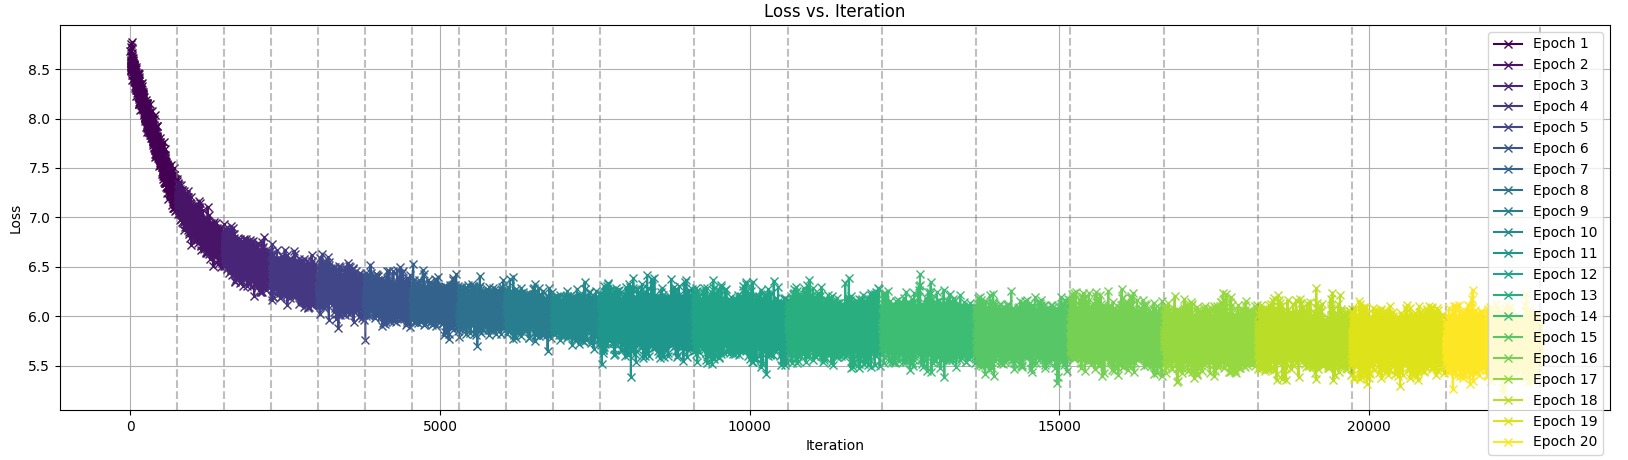
\includegraphics[width=0.95\linewidth]{1.png}}
    \caption{Απώλεια με Κωδικοποίηση Θέσης, 8 Κεφαλές, 6 Επίπεδα Αποκωδικοποίησης}
\end{figure}


\subsection{Απώλεια με Κωδικοποίηση Θέσης και 2 Κεφαλές, 3 Επίπεδα Αποκωδικοποίησης}

Η εικόνα δείχνει την απώλεια κατά την εκπαίδευση του μοντέλου με κωδικοποίηση θέσης, 2 κεφαλές και 3 επίπεδα αποκωδικοποίησης. Η απώλεια επίσης μειώνεται σταθερά, αλλά με λιγότερες κεφαλές και επίπεδα αποκωδικοποίησης.


\begin{figure}[htbp]
    \centerline{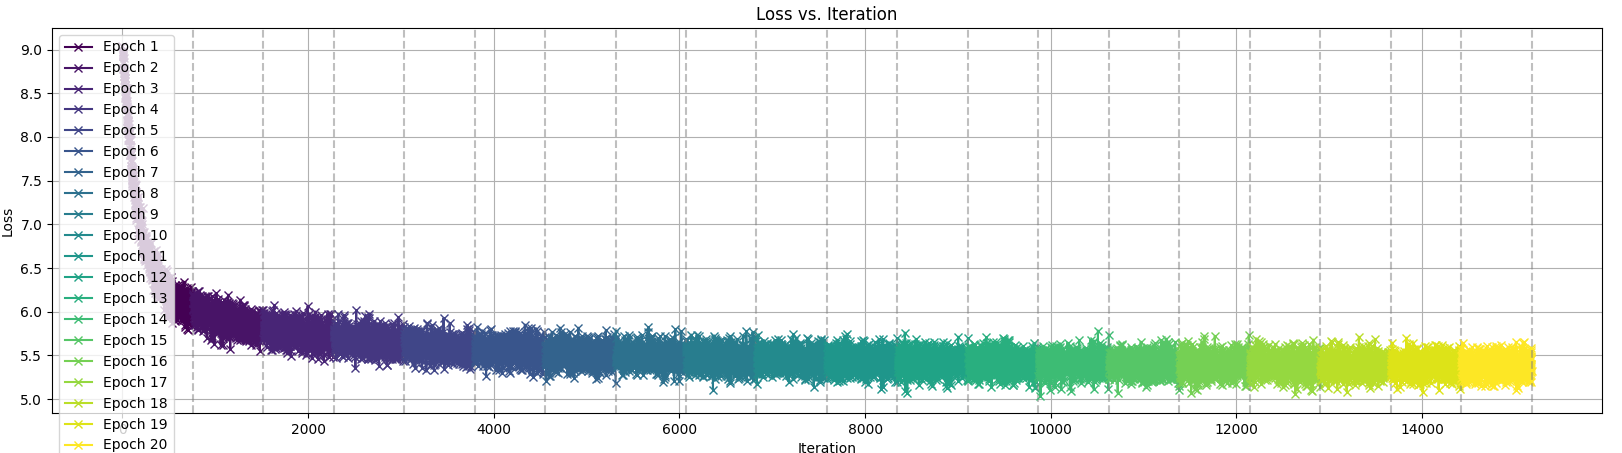
\includegraphics[width=0.95\linewidth]{2.png}}
    \caption{Απώλεια με Κωδικοποίηση Θέσης, 2 Κεφαλές, 3 Επίπεδα Αποκωδικοποίησης}
\end{figure}


\subsection{Απώλεια με \textlatin{GRU}}

Οι παρακάτω εικόνες παρουσιάζουν την απώλεια κατά την εκπαίδευση αλλά και του \textlatin{validation} του μοντέλου χρησιμοποιώντας \textlatin{GRU}. Παρατηρείται οτι οσο και αυξανω το βάθος ή ανεβάζω το μέγεθος του embedding, δεν υπάρχει κάποια βελτίωση στην απώλεια. 


\begin{figure}[htbp]
    \centerline{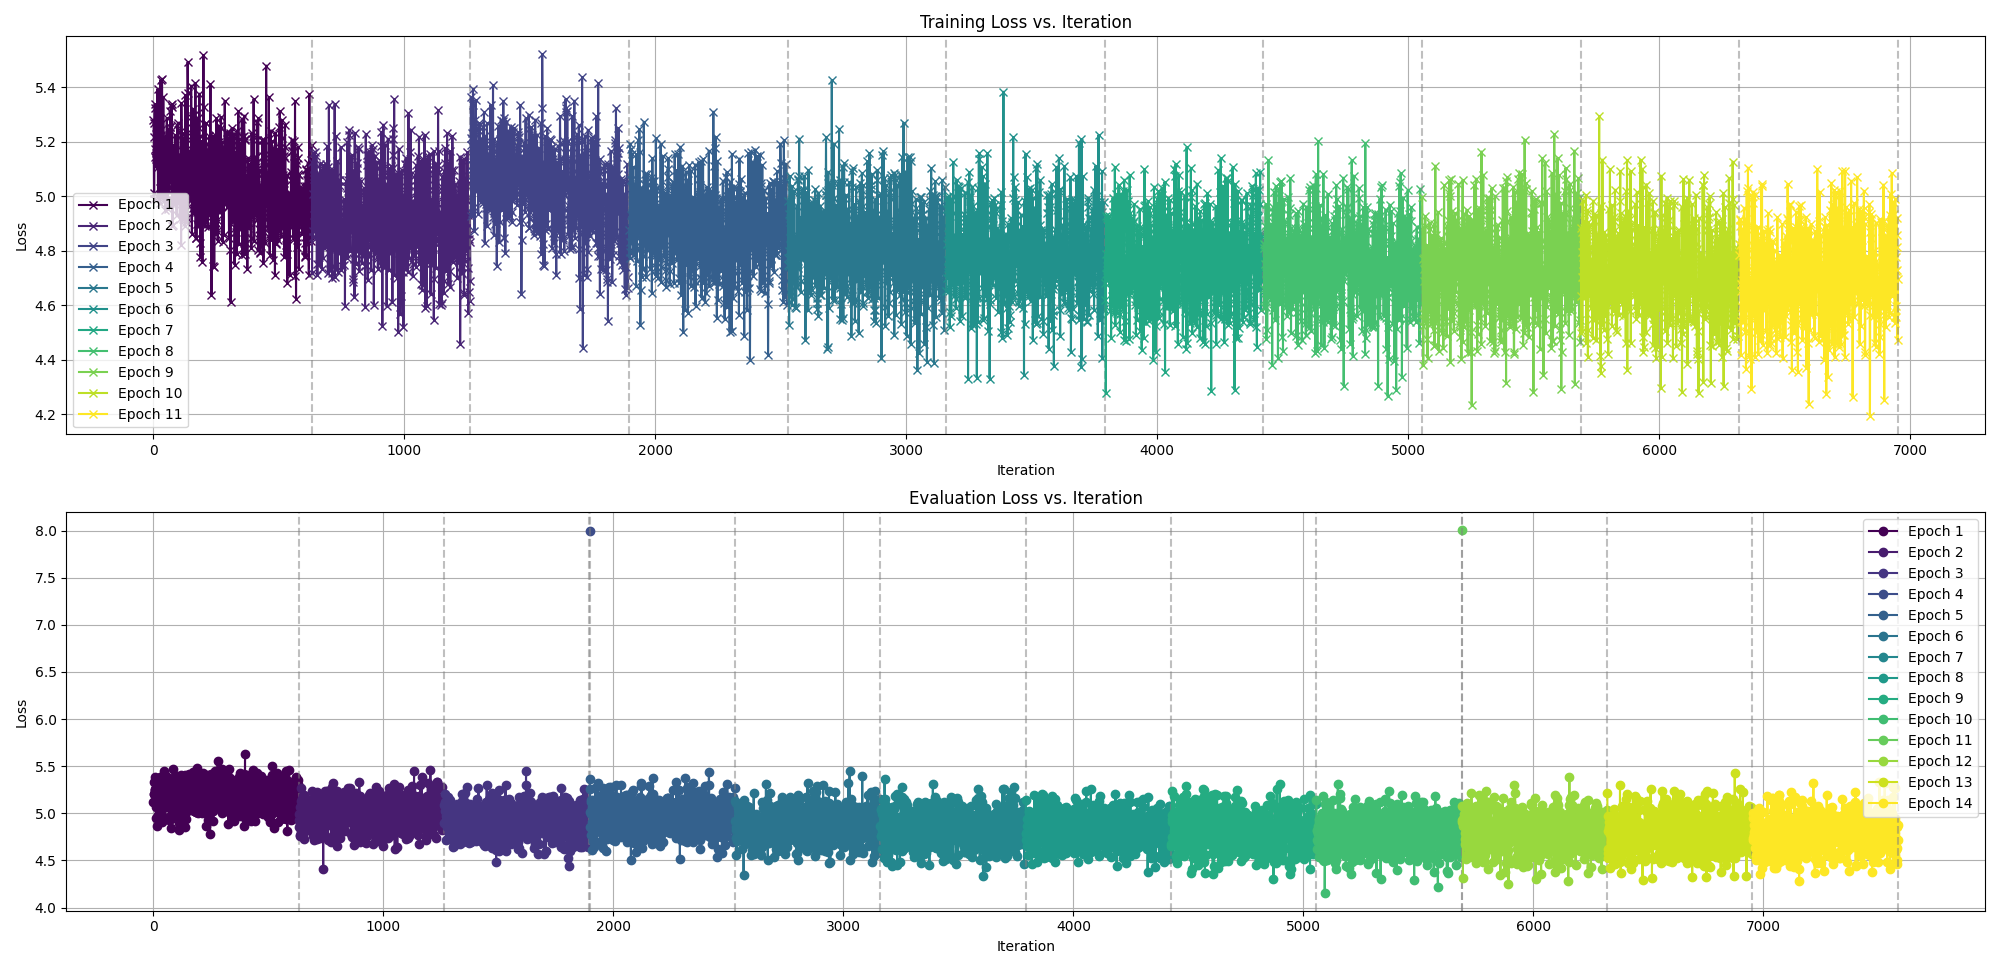
\includegraphics[width=0.95\linewidth]{gru 8layers 512hidden.png}}
    \caption{Απώλεια με \textlatin{GRU 8 layers 512 hidden}}
\end{figure}

\begin{figure}[htbp]
    \centerline{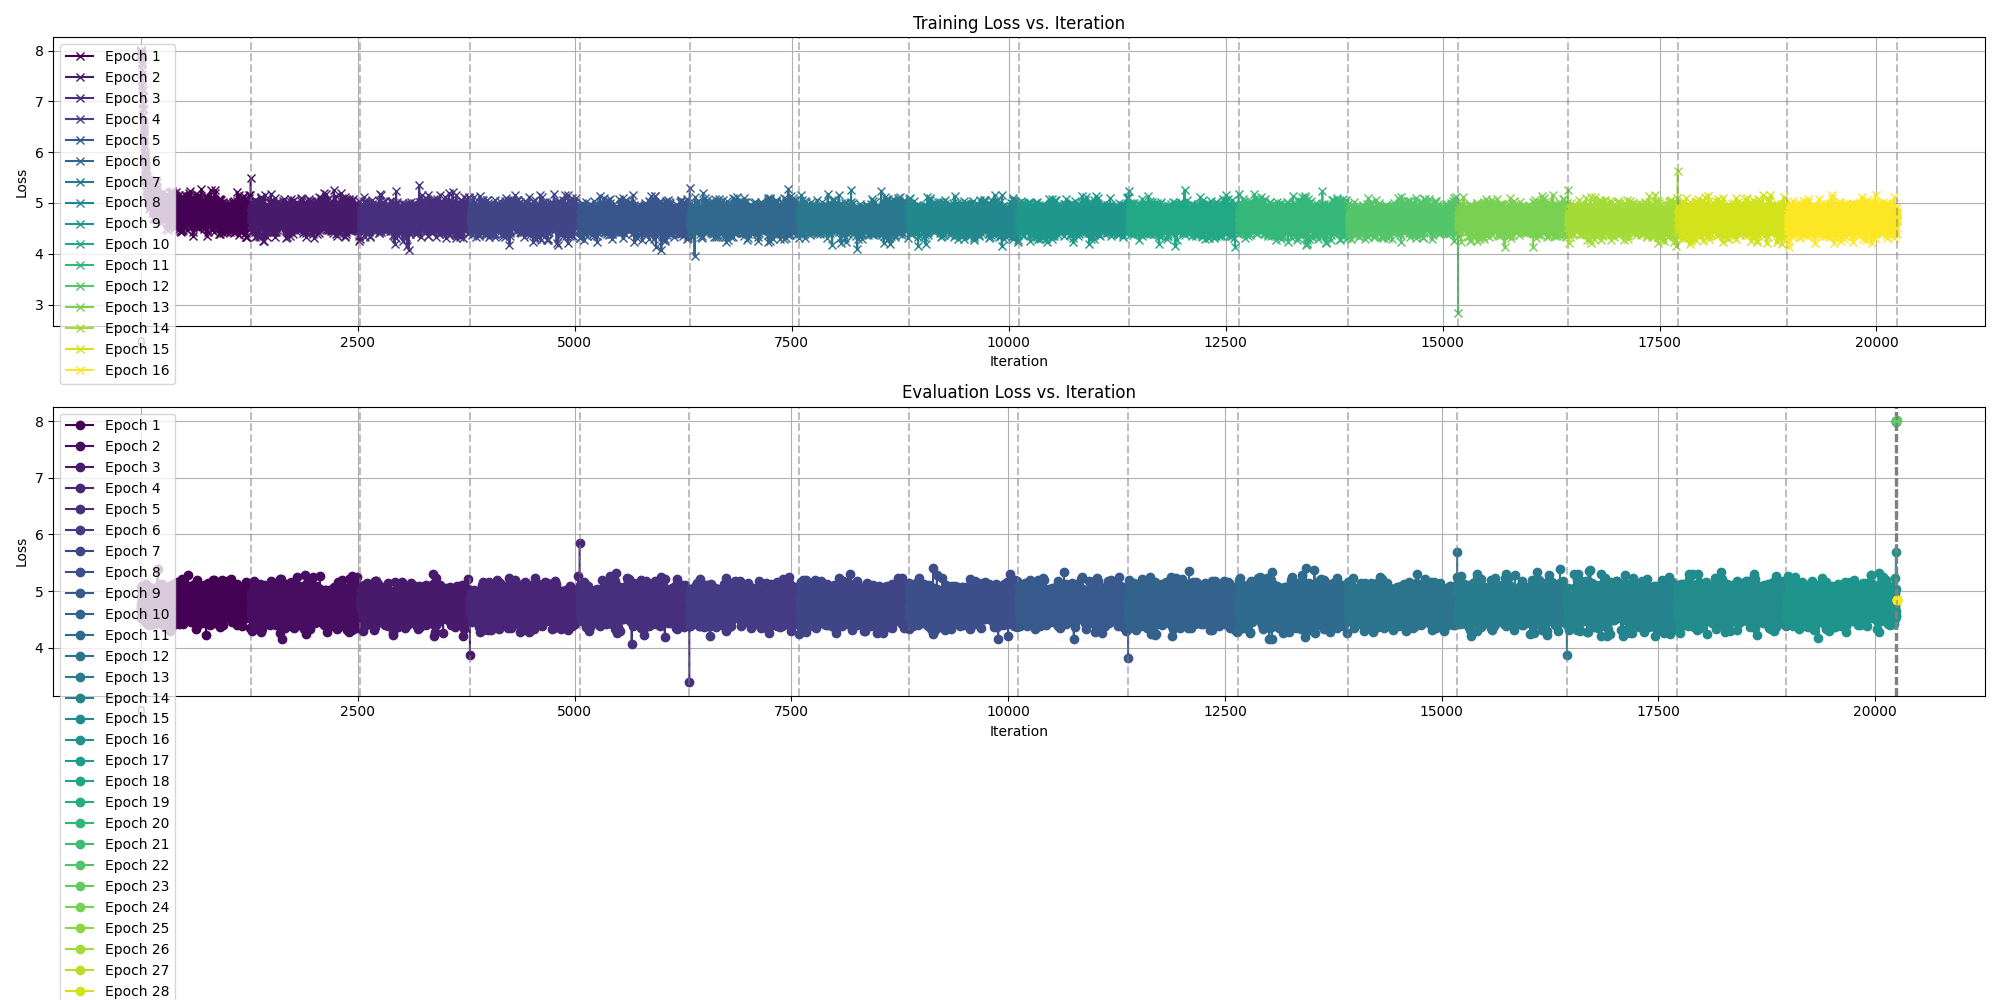
\includegraphics[width=0.95\linewidth]{gru 16layers 4098 embed.png}}
    \caption{Απώλεια με \textlatin{GRU 16 layers 4098 embedding}}
\end{figure}

\begin{figure}[htbp]
    \centerline{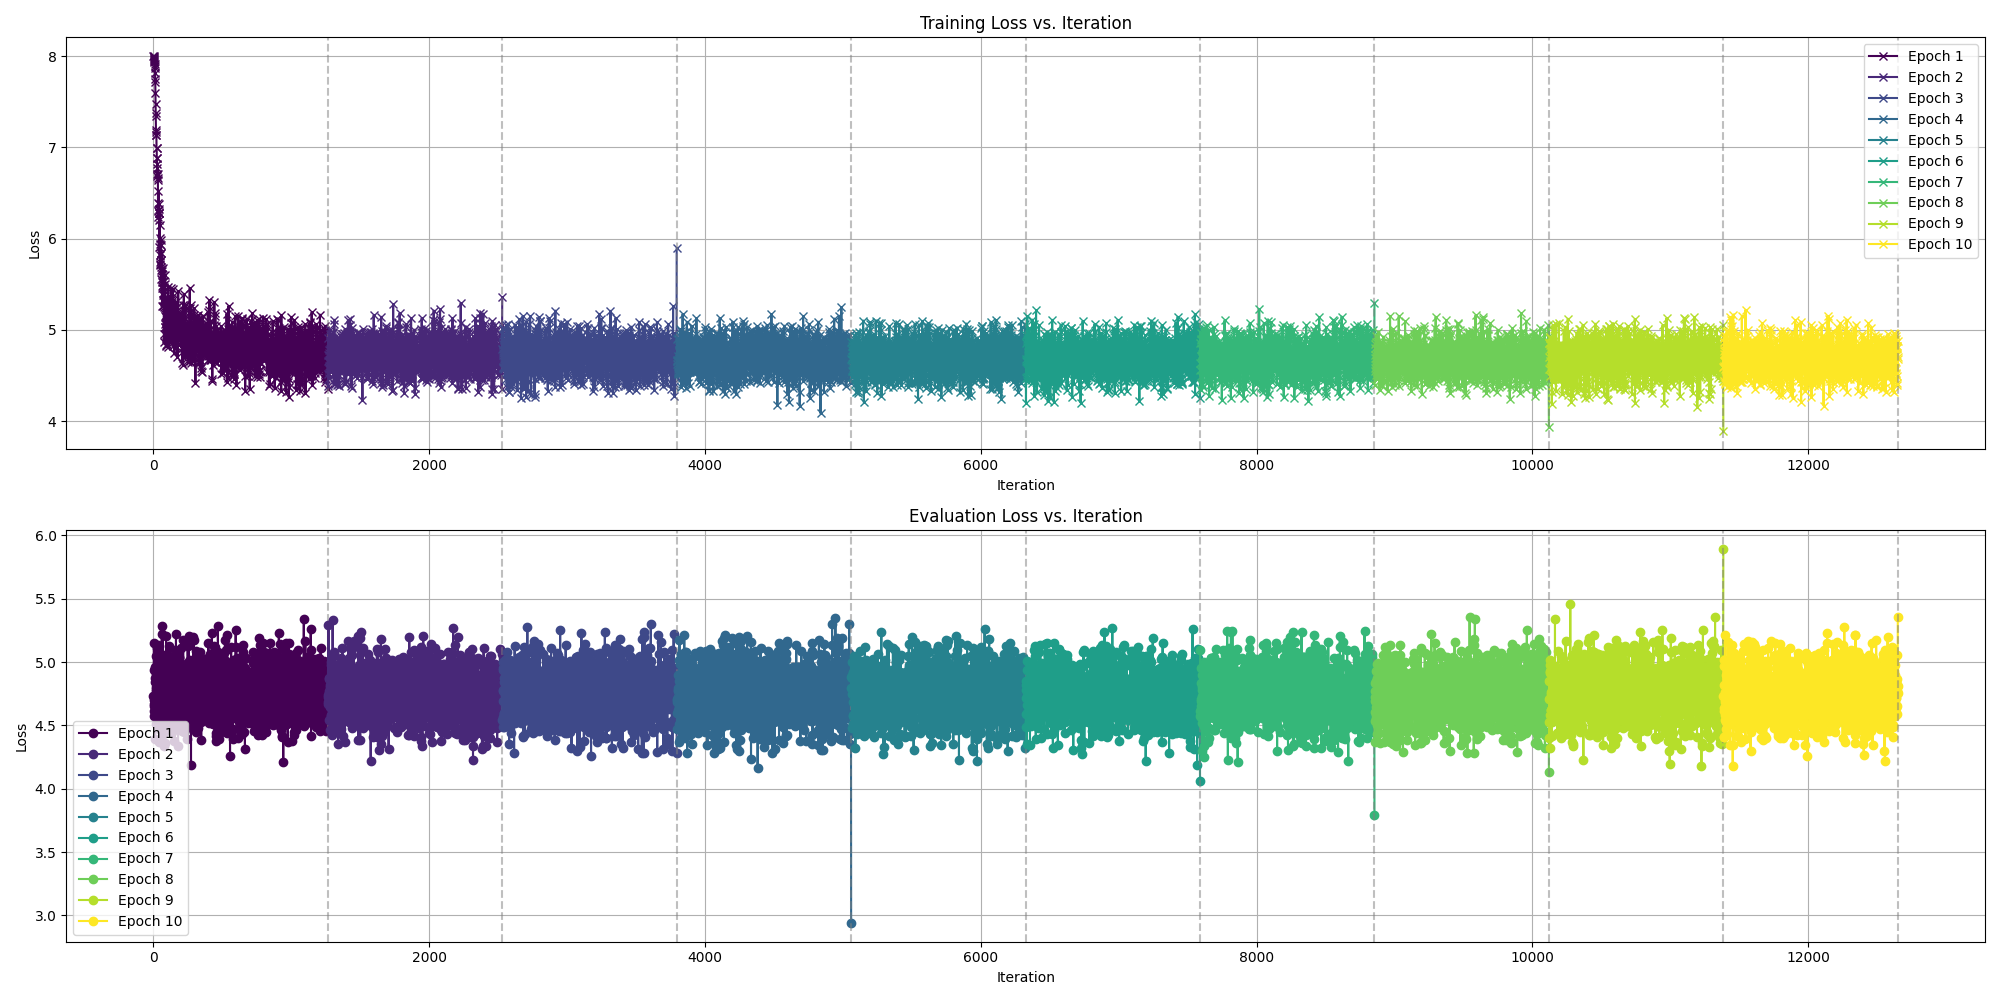
\includegraphics[width=0.95\linewidth]{gru 64 layers 1024 emb.png}}
    \caption{Απώλεια με \textlatin{GRU 64 layers 1024 embedding}}
\end{figure}


\subsection{Υπόλοιπες αρχιτεκτονικές}

Αποφάσησα να μην εμφανισω άλλες εικόνες με loss καθώς είχαν παρθεί από όταν δεν είχα φτιάξει το πρόβλημα που εμφανίστηκε με τον data loader. Παράδειγμα αυτών η παρακάτω εικόνα.

Παρακάτω η εικόνα παρουσιάζει την απώλεια κατά την εκπαίδευση του μοντέλου με κωδικοποίηση θέσης, 16 κεφαλές και 32 επίπεδα αποκωδικοποίησης. Παρατηρείται υπερεκπαίδευση (\textlatin{overfitting}), καθώς δεν είχα ακόμει φτίαξει κατάλληλα τον \textlatin{data loader} για να αποφύγω την υπερεκπαίδευση και υπηρχαν εικονες που εμφανιζοντουσαν και στα 2 \textlatin{data loaders test / train}.

\begin{figure}[htbp]
    \centerline{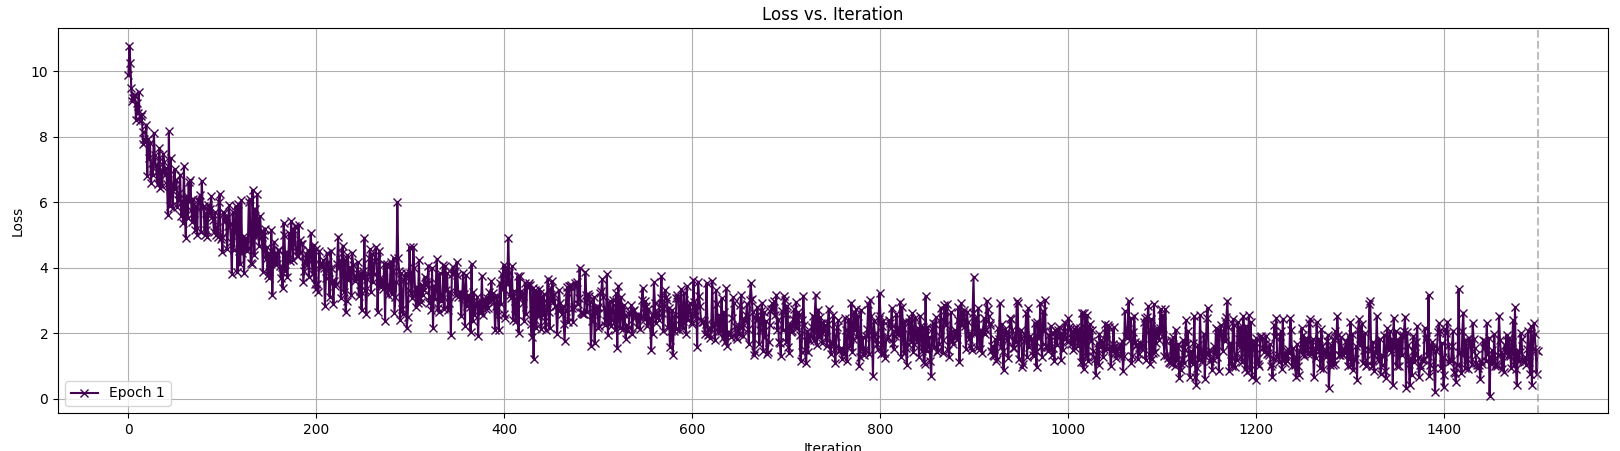
\includegraphics[width=0.8\linewidth]{3.png}}
    \caption{Απώλεια με Κωδικοποίηση Θέσης, 16 Κεφαλές, 32 Επίπεδα Αποκωδικοποίησης (1), αποτέλεσμα overfitting}
\end{figure}

\subsection{Συμπεράσματα}

Σαν αποτέλεσμα δεν είχα κάποια ιδιαίτερη επιτυχία στην μείωση της απώλειας και την βελτίωση του μοντέλου. Το μοντέλο βγάζει αποτελέσματα αλλά δεν έχουν κάποια σημασία ή συνοχή. Παρόλα αυτά η εμπειρία αυτή με βοήθησε να καταλάβω καλύτερα την λειτουργία των συνελεκτικών και αναδρομικών δικτύων και την διαδικασία εκπαίδευσης τους. 

\end{document}
